% chapter3_1.tex -- de (German)
% installation of Raspbian Buster Lite
\section{\os{Raspbian Buster Lite} auf dem {\RPi} installieren}
Einige Tutorials im Internet empfehlen zwar, die Software f�r die
{\Bezeichnung} unter \os{Raspbian Buster with desktop} zu installieren,
aber da es sich bei der {\Bezeichnung} um ein einfaches
stand\-alone-System ohne Bildschirm handelt, ist es in meinen Augen
v�llig ausreichend, die Installation auf dem wesentlich kleineren
\os{Raspbian Lite} vorzunehmen. Ein grafischer X11-Desktop ist
schlichtweg nicht erforderlich. Au�erdem reicht f�r \os{Raspbian Buster
Lite} zur Not sogar eine SD-Karte mit einer Speicherkapazit�t von 4GB.

\subsection{Erstellen einer SD-Karte mit \os{Raspbian Buster Lite}}
Zun�chst wird die aktuelle Version von \os{Raspbian Buster Lite} von der
Homepage der {\foundation}
(\url{https://www.raspberrypi.org/downloads/raspbian/}, ca. 450MiB)
heruntergeladen und entpackt (1,8GiB). Das entpackte Image wird mit
einem daf�r vorgesehenen Programm wie \software{win32diskimager} oder
am Linux-PC mit dem systemeigenen Kommando \cmd{dd} auf die SD-Karte
\textit{geflasht}, um das Image 1:1 zu �bertragen.
\begin{bclogo}[arrondi = 0.2, logo = \bcinfo, ombre = true, epOmbre = 0.25, couleurOmbre = black!30,blur]{Achtung}
Es reicht nicht, die Imagedatei einfach auf eine bereits formatierte
SD-Karte zu kopieren!
\end{bclogo}
Die Details des \textit{Flashens} von Betriebssystem-Images auf eine
SD-Karte werden von der {\foundation} unter
\url{https://www.raspberrypi.org/documentation/installation/installing-images/README.md}
ausf�hrlich beschrieben und in diesem Dokument als bekannt
vorausgesetzt.

Nach dem Flashen enth�lt die SD-Karte zwei Partitionen:
\begin{compactitem}
\item{die FAT32-formatierte \filenam{/boot}-Partition}
\item{die ext4-formatierte Rootpartition von \os{Raspbian}}
\end{compactitem}
\begin{bclogo}[logo = \bclampe, noborder = true]{Hinweis}
Beim (erneuten) Anstecken der SD-Karte am PC werden diese beiden
Partitionen im Dateimanager angezeigt. Sollte auf dem PC jedoch das
Betriebssystem \os{Windows} verwendet werden, so wird nur die
FAT32-formatierte \filenam{/boot}-Partition erkannt.
\end{bclogo}


\newpage
\subsection{Anmeldung am {\RPi} �ber \software{ssh}}
\begin{bclogo}[logo = \bclampe, noborder = true]{Hinweis}
F�r die ersten Schritte muss die Netzwerkverbindung zum {\RPi} �ber ein
verkabeltes LAN aufgebaut werden, da die WLAN-Verbindung noch nicht
eingerichtet ist! Dies geschieht erst in Abschnitt \ref{sect:setupWLAN}.
\end{bclogo}
\begin{figure}[h]
\centering
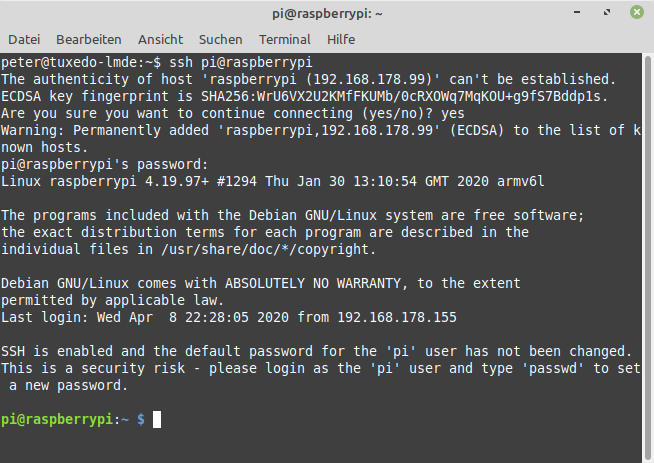
\includegraphics[width=0.90\textwidth, angle=0]{software/login.png}
\caption{erster Login �ber \software{ssh}}
\label{fig:ssh_login}
\end{figure}
Da an den {\RPi} f�r die {\Bezeichnung} weder Bildschirm noch Tastatur
angeschlossen werden, muss der Zugriff auf den {\RPi} von Anfang an �ber
\software{ssh} erfolgen. Dazu muss auf der Partition \filenam{/boot} der
SD-Karte die leere Datei \filenam{ssh} angelegt werden.\\
Nun wird die SD-Karte in den {\RPi} gesteckt, der {\RPi} \textbf{�ber
Ethernet ans LAN} geh�ngt und eingeschaltet. Nach sp�testens einer Minute
sollte \os{Raspbian Buster Lite} vollst�ndig gebootet und der {\RPi} im
LAN bekannt sein. Auf dem PC wird in einem Terminalfenster
(unter \os{Windows} in der Eingabeaufforderung \cmd{cmd.exe}) die
Software \software{ssh} mit folgendem Kommando gestartet:

\cmdPC{ssh pi@raspberrypi}\comment{Das Passwort lautet \texttt{raspberry}}

Die Bildschirmausgabe sieht in etwa wie in Abbildung \ref{fig:ssh_login}
aus.


\newpage
\subsection{\os{Raspbian} konfigurieren}
Nach erfolgreichem \software{ssh}-Login muss das System jetzt auf einen
aktuellen und sicheren Stand gebracht werden:\\
\cmdPi{sudo apt update \&\& sudo apt upgrade}\comment{System auf den neuesten Stand bringen}\\
\cmdPi{sudo raspi-config}\\
\stdout{1 Change User Password \ \ \ \ \ \ \ \ \ \ \ \ \ \ \ \ \ \ \ \ \ \ \ \ \ \ \ }\comment{Passwort unbedingt �ndern!}\\
\stdout{2 Network Options \ \ \ \ \ --> N1 Hostname \ \ \ \ \ \ \ \ \ \ \ \ }\comment{\zB \texttt{phoniebox1}}\\
\stdout{3 Boot Options \ \ \ \ \ \ \ \ --> B1 Desktop / CLI \ \ \ \ \ \ \ \ --> B2 Console Autologin}\\
%\stdout{4 Localisation Options --> I1 Change Locale \ \ \ \ \ \ \ }\comment{Landeseinstellungen}\\
\stdout{4 Localisation Options --> I2 Change Timezone \ \ \ \ \ }\comment{Zeitzone anpassen}\\
\stdout{\textcolor{white}{ \ \ \ \ \ \ \ \ \ \ \ \ \ \ \ \ \ \ \ \ \ \ } --> I4 Change Wi-fi Country }\comment{diese Anpassung ist ganz wichtig!}\\
\stdout{5 Interfacing Options \ --> P2 SSH}

Beim Verlassen von \software{raspi-config} sollte die Abfrage 
\texttt{Would you like to reboot now?} mit \button{yes} beantwortet
werden. Der {\RPi} wird neu hochgefahren. Vom PC aus kann nach ca.
einer Minute Wartezeit ein neuer \software{ssh}-Login auf den neuen
Hostnamen mit dem (hoffentlich) ge�nderten Passwort erfolgen:\\
\cmdPC{ssh pi@phoniebox1}

\subsection{WLAN einrichten}
\label{sect:setupWLAN}
Da die {\Bezeichnung} als tragbares Ger�t f�r's Kinderzimmer konzipiert
ist, sollte ein WLAN-Zu\-gang eingerichtet werden, um als Eltern sp�ter
\zB per Laptop oder Smartphone jederzeit einen \textit{bequemen}
Zugriff auf die Box zu haben. Wie h�ufig unter \os{Linux} gibt es auch
f�r die WLAN-Konfiguration mehrere zielf�hrende Wege, wie sie \zB im
Elek\-tro\-nik-Kom\-pen\-dium unter
\url{https://www.elektronik-kompendium.de/sites/raspberry-pi/1912221.htm}
beschrieben werden. F�r {\autor}s {\Bezeichnung} wird die dort
beschriebene "`Variante 2"' mittels \software{wpa\_supplicant}
verwendet.

Auf einem frisch installierten \os{Raspbian Lite} wird der WLAN-Zugriff
in der \software{ssh}-Konsole  �ber die Datei
\filenam{ /etc/wpa\_supplicant/wpa\_supplicant.conf} eingerichtet. Die
drei ersten Zeilen sollten in der Datei bereits vorhanden sein. F�r
jedes gew�nschte WLAN muss ein Eintrag \texttt{network\{\dots\}} nach
folgendem Schema eingef�gt werden. Dazu wird der auch �ber
\software{ssh} funktionierende Texteditor \software{nano} verwendet:\\
\cmdPi{sudo nano /etc/wpa\_supplicant/wpa\_supplicant.conf}\\
\editor{ctrl\_interface=DIR=/var/run/wpa\_supplicant GROUP=netdev\\
        update\_config=1\\
        country=DE\\
        \\
        network=\{ \# Erweiterungen von \autor\\
        \textcolor{white}{\ \ \ \ }ssid="{<wlan-name>}" \ \# Klartext-Bezeichnung des Netzwerkes\\
        \textcolor{white}{\ \ \ \ }psk="{<passphrase>}" \ \# Passwort f�r WLAN-Zugriff\\
        \textcolor{white}{\ \ \ \ }key\_mgmt=WPA-PSK\\
        \}
       }
       
Um diese Einstellungen tats�chlich zu aktivieren, m�ssen im Anschluss
folgende Kommandos abgesetzt werden:\\
\cmdPi{sudo systemctl restart dhcpcd}\\
\stdout{\textcolor{red}{Warning:} The unit file, source configuration
        file or drop-ins of dhcpcd.service changed on disk. Run
        'systemctl daemon-reload' to reload units.}\\
\cmdPi{sudo systemctl daemon-reload}\comment{gem�� obiger Warnung}\\
\cmdPi{ip addr}\\
\stdout{1: lo: <LOOPBACK\,UP\,LOWER\_UP> mtu 65536 qdisc noqueue state UNKNOWN group default qlen 1000\\
        \textcolor{white}{\ \ \ \ }link/loopback 00:00:00:00:00:00 brd 00:00:00:00:00:00\\
        \textcolor{white}{\ \ \ \ }inet 127.0.0.1/8 scope host lo\\
        \textcolor{white}{\ \ \ \ \ \ \ }valid\_lft forever preferred\_lft forever\\
        \textcolor{white}{\ \ \ \ }inet6 ::1/128 scope host\\
        \textcolor{white}{\ \ \ \ \ \ \ }valid\_lft forever preferred\_lft forever\\
        2: eth0: BROADCAST\,MULTICAST\,UP\,LOWER\_UP> mtu 1500 qdisc pfifo\_fast state UP group default qlen 1000\\
        \textcolor{white}{\ \ \ \ }link/ether b8:27:eb:36:6f:a7 brd ff:ff:ff:ff:ff:ff\\
        \textcolor{white}{\ \ \ \ }inet 192.168.178.153/24 brd 192.168.178.255 scope global dynamic noprefixroute eth0\\
        \textcolor{white}{\ \ \ \ \ \ \ }valid\_lft 859570sec preferred\_lft 751570sec\\
        \textcolor{white}{\ \ \ \ }inet6 fe80::3a9f:9d8c:1f44:e940/64 scope link \\
        \textcolor{white}{\ \ \ \ \ \ \ }valid\_lft forever preferred\_lft forever\\
        3: wlan0: <BROADCAST\,MULTICAST\,UP\,LOWER\_UP> mtu 1500 qdisc pfifo\_fast state UP group default qlen 1000\\
        \textcolor{white}{\ \ \ \ }link/ether b8:27:eb:63:3a:f2 brd ff:ff:ff:ff:ff:ff\\
        \textcolor{white}{\ \ \ \ }inet 192.168.178.154/24 brd 192.168.178.255 scope global dynamic noprefixroute wlan0\\
        \textcolor{white}{\ \ \ \ \ \ \ }valid\_lft 863877sec preferred\_lft 755877sec\\
        \textcolor{white}{\ \ \ \ }inet6 fe80::b04c:315b:a4c9:3c9d/64 scope link\\
        \textcolor{white}{\ \ \ \ \ \ \ }valid\_lft forever preferred\_lft forever
       }

Damit ist die {\Bezeichnung} f�r den k�nftigen WLAN-Zu\-griff
freigeschaltet. Der bis jetzt verwendete LAN-Zu\-griff �ber das
Ethernetkabel ist ab sofort nicht mehr notwendig. Zum Test wird die
laufende \software{ssh}-Sitzung beendet, das Ethernetkabel abgesteckt
und eine neue \software{ssh}-Sitzung gestartet:\\
\cmdPi{exit}\comment{Schlie�en der bestehenden ssh-Sitzung �ber LAN}\\
\textit{Jetzt das Ethernetkabel abstecken!}\\
\cmdPC{ssh pi@phoniebox1}\comment{neue ssh-Sizung �ber WLAN �ffnen}

%\begin{bclogo}[arrondi = 0.2, logo = \bcinfo, ombre = true, epOmbre = 0.25, couleurOmbre = black!30,blur]{Achtung}
\begin{bclogo}[logo = \bclampe, noborder = true]{Hinweis}
Entgegen vieler Tutorials wurde bei {\autor}s {\Bezeichnung} auf die
Zuteilung einer statischen (festen) IP-Adresse verzichtet! Stattdessen
wird von der {\Bezeichnung} beim Bootvorgang �ber DHCP eine dynamische
IP-Adresse angefordert, um den Netzwerkzugriff m�glichst flexibel zu
halten. Die konkret vergebene IP-Adresse kann mit dem Kommando
\cmd{ip addr} ermittelt werden und lautet im obigen Beispiel
\texttt{192.168.178.154}.
\end{bclogo}
